\documentclass[11pt,spanish,a4paper]{article}
% Versión 2.o cuat 2015 Víctor Bettachini < bettachini@df.uba.ar >

\usepackage{babel}
\addto\shorthandsspanish{\spanishdeactivate{~<>}}
\usepackage[utf8]{inputenc}
\usepackage{float}

\usepackage{units}
\usepackage[separate-uncertainty=true, multi-part-units=single, locale=FR]{siunitx}

\usepackage{amsmath}
\usepackage{amstext}
\usepackage{amssymb}

\newcommand{\pvec}[1]{\vec{#1}\mkern2mu\vphantom{#1}}

% \usepackage{tikz}
% \input{DimLinesTikz}
% \usetikzlibrary{decorations.pathmorphing, patterns}

\usepackage{graphicx}
\graphicspath{{./graphs/}}

\usepackage[margin=1.3cm,nohead]{geometry}
% \voffset-3.5cm
% \hoffset-3cm
% \setlength{\textwidth}{17.5cm}
% \setlength{\textheight}{27cm}

\usepackage{lastpage}
\usepackage{fancyhdr}
\pagestyle{fancyplain}
\fancyhead{}
\fancyfoot{{\tiny \textcopyright Departamento de Física, FCEyN, UBA}}
\fancyfoot[C]{ {\tiny Actualizado al \today} }
\fancyfoot[RO, LE]{Pág. \thepage/\pageref{LastPage}}
\renewcommand{\headrulewidth}{0pt}
\renewcommand{\footrulewidth}{0pt}

% \def \materia {Física II para químicos}
\def \periodo {cuatrimestre de verano - 2017}
\def \website {http://materias.df.uba.ar/f2qa2017v}


\begin{document}
\noindent
\textbf{Física II (Químicos)}\hfill \textcopyright {\tt DF, FCEyN, UBA}
% \textbf{\materia}\hfill \periodo
\begin{center}
  \textsc{\large Magnetostática - Ley de Ampère - Momento magnético - Medios magnéticos}
  % \textsc{\large Guía 4: Magnetostática - Ley de Ampère - Momento magnético - Medios magnéticos}
\par\end{center}{\large \par}


\begin{enumerate}
% \begin{description}

\section*{Magnetostática}

  \item Una partícula de carga \(q\) se mueve en un campo magnético uniforme \(\vec{B}\) con una velocidad \(\vec{v}\)
  % \item[Problema 1] Una partícula de carga \(q\) se mueve en un campo magnético uniforme \(\vec{B}\) con una velocidad \(\vec{v}\)
perpendicular al campo.
\begin{enumerate}
  \item  Calcule el radio de la órbita circular descripta.
¿Aumenta el módulo de la velocidad?¿Por qué?
  \item Determine la frecuencia del movimiento circular descripto.
  \item ¿Qué sucede si la velocidad es paralela al campo magnético? ¿Y si tiene una componente
paralela al campo y otra perpendicular?
\end{enumerate}

 
  \item \begin{minipage}[t]{0.65\textwidth}
		 Una partícula de carga \(q\) entra, con una velocidad \(\vec{v}\) , en una región del espacio donde existe un campo eléctrico uniforme \(\vec{E}\) de \SI{80}{\kilo\volt\per\metre} dirigido hacia abajo, como se muestra en la figura.
Perpendicular al campo eléctrico y a la velocidad de la partícula cargada, se halla un campo magnético \(\vec{B}\) de \SI{0,4}{\tesla}.
Si la rapidez de la partícula se escoge apropiadamente, ésta no sufrirá ninguna deflexión a causa de los campos perpendiculares.
¿Qué rapidez debe ser seleccionada en este caso? (Este dispositivo se llama selector de velocidades)
	\end{minipage}
	\begin{minipage}[c][1em][t]{0.3\textwidth}
			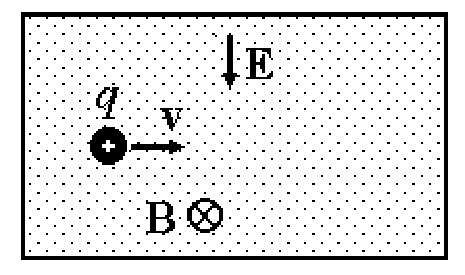
\includegraphics[width=\textwidth]{p4e02}
	\end{minipage}


  \item \begin{minipage}[t]{0.7\textwidth}
  La figura muestra un dispositivo empleado para la medición de la masa de los iones.
Un ion de masa \(m\) y carga \(+q\) sale esencialmente en reposo de la fuente \(S\), cámara donde se produce la descarga de un gas.
La diferencia de potencial \(V\) acelera el ion y se permite que entre en una región con un campo magnético perpendicular uniforme \(\vec{B}\).
Dentro del campo, el ion se mueve en semicírculo, chocando con una placa fotográfica a la distancia \(x\) de la rendija de entrada.
Demuestre que la masa m del ion está dada por 
\[
  m= \frac{B^2 q}{8 V} x^2
\]
	\end{minipage}
	% \begin{minipage}{0.25\textwidth}
	\begin{minipage}[c][1em][t]{0.25\textwidth}
  		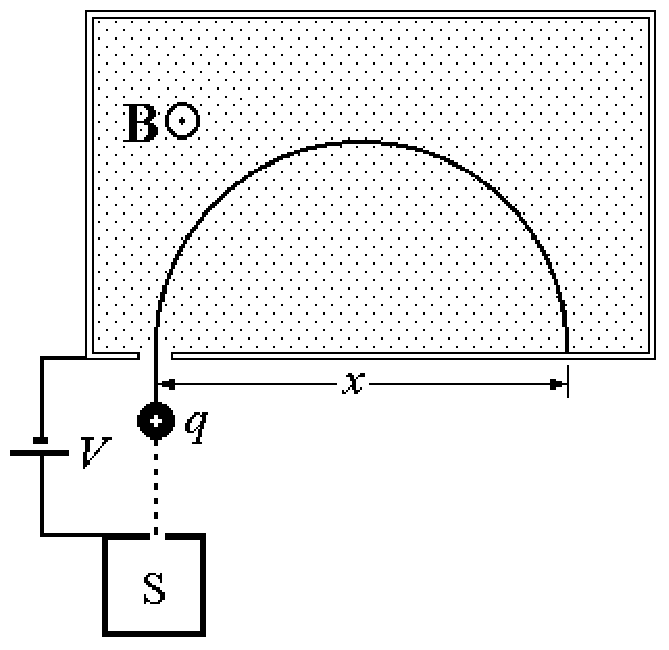
\includegraphics[width=\textwidth]{p4e03}
	\end{minipage}


\section*{Ley de Ampère}

  \item Calcule la fuerza por unidad de longitud entre dos cables paralelos por los que circula una corriente de \SI{30}{A}.
La separación entre cables es de \SI{2}{\centi\metre}.
Estime hasta qué distancia por encima de los cables se verá afectada la indicación de una brújula.
Considere los dos posibles sentidos de circulación de la corriente.
Suponga que la intensidad del campo magnético terrestre en el lugar es de \SI{5E-4}{\tesla} y forma un ángulo de \SI{30}{\degree} con la vertical.


  \item Dibuje cualitativamente las líneas de campo magnético correspondientes a dos cables rectilíneos infinitos y paralelos, que conducen sendas corrientes \(I\) de sentido contrario.
Tenga en cuenta cuál debe ser el comportamiento del campo cerca y lejos de los cables.


  \item Aprovechando la simetría de la distribución de corrientes y usando la ley de Ampère, determine el vector campo magnético en los siguientes casos:
\begin{enumerate}
\item un cable rectilíneo infinito por el que circula una corriente \(I\),
\item un cilindro infinito de radio \(R\) por el que circula una densidad de corriente uniforme \(j\),
\item un solenoide infinito de \(n\) vueltas por unidad de longitud y corriente \(I\) (suponga que el devanado es suficientemente denso como para despreciar la componente longitudinal de los elementos de corriente),
\item un plano infinito con densidad superficial de corriente g uniforme,
\item dos planos infinitos paralelos, separados una distancia d, con densidades de corriente uniformes \(g\) y \(-g\),
\item una lámina infinita de caras plano-paralelas y espesor \(d\), con densidad de corriente \(j\) uniforme,
\item un toroide de radio interior \(a\) y radio exterior \(b\), con un arrollamiento denso de \(N\) vueltas por el que circula una corriente \(I\).
\end{enumerate}


\section*{Momento magnético}

  \item \setlength{\parskip}{0cm}
  \begin{enumerate}
  \item Calcule el campo magnético sobre el eje de una espira circular de área \(A\) y corriente \(I\).
  \item Repita el cálculo para una espira cuadrada.
  \item  Estudie y compare los comportamientos de ambos resultados para distancias grandes.
Expréselos en función de los momentos magnéticos de las espiras. 
\end{enumerate}


  \item \setlength{\parskip}{0cm}
\begin{enumerate}
  \item Calcule el campo magnético sobre el eje de un solenoide de longitud \(L\), con \(N\) vueltas devanadas densamente, por el que circula una corriente \(I\). 
  \item Estudie el comportamiento a grandes distancias y encuentre el valor del momento
magnético del solenoide.
  \item Obtenga el límite de solenoide infinito.
  \item Suponga que el solenoide tiene \SI{40}{\centi\metre}de largo, \SI{10}{\centi\metre} de diámetro y el campo en el centro es de \SI{3}{\tesla} (éste es un campo muy intenso).
Si el solenoide se encuentra en el subsuelo del pabellón I, ¿influirá en la medición del campo magnético terrestre que realizan los alumnos en el segundo piso?
\end{enumerate}


  \item Calcule la fuerza sobre una aguja pequeña magnetizada con momento magnético \(\vec{m}\), colocada sobre el eje del solenoide finito del problema anterior.
Exprese la fuerza en función de la distancia al centro del solenoide.
Discuta el sentido de la fuerza en relación a los sentidos del momento magnético \(\vec{m}\) y el campo magnético \(\vec{B}\).



\section*{Medios magnéticos}
  \vspace{-1cm}
  \item \begin{minipage}[t]{0.7\textwidth}
	Un cable coaxial está formado por dos conductores cilíndricos coaxiales separados por un medio de permeabilidad \(\mu\) (ver figura).
	Por ambos conductores circulan corrientes \(I\) iguales y opuestas.
	Suponiendo que la densidad de corriente en cada uno de los conductores es uniforme, encuentre el campo magnético \(\vec{B}\) en todo punto del espacio.
	\end{minipage}
	\begin{minipage}[c][7em][t]{0.25\textwidth}
  		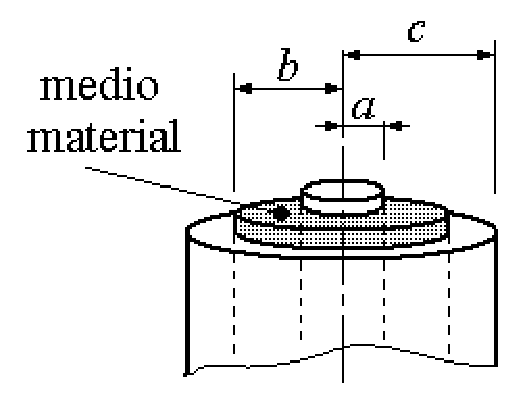
\includegraphics[width=\textwidth]{p4e10}
	\end{minipage}


\item Un cilindro infinito de radio a es circulado por una corriente volumétrica uniforme \(\vec{j}= j_0 \hat{z}\), coaxial con el cilindro.
% \item[Problema 11] Un cilindro infinito de radio a es circulado por una corriente volumétrica uniforme \(\vec{j}= j_0 \hat{z}\), coaxial con el cilindro.
En la zona \(b < r < c\, (a < b)\), se tiene un medio magnético lineal, isótropo y homogéneo cuya permeabilidad relativa es \(\mu_r= 1000\).
\begin{enumerate}
\item Calcular los campos H y B en todo el espacio.
\item ¿Se comporta el medio material como un blindaje magnético? 
\end{enumerate}


\end{enumerate}
% \end{description}
\end{document}
